\vspace{0ex}
\chapter {PENDAHULUAN}

Pada bab ini, akan dijelaskan mengenai latar belakang, rumusan masalah, batasan masalah, tujuan, metodologi pengerjaan, dan sistematika penulisan Tugas Akhir.

\section{Latar Belakang}

\par \CG adalah cabang dari ilmu komputer yang dikhususkan untuk mempelajari algoritma yang dapat dinyatakan dalam suatu geometri. Salah satu algoritma yang sering dipakai pada \CG adalah algoritma \CG. \CH adalah sebuah set poligon dari titik pada bidang Euclidean atau ruang Euclidean, atau dapat disebut himpunan cembung terkecil yang berisi titik. Sebagai contoh, ketika suatu kumpulan titik merupakan bagian yang dibatasi dalam sebuah bidang, \CH dapat divisualisasikan sebagai bentuk yang tertutup oleh karet gelang yang membentang di sekitar titik - titik tersebut. Berikut merupakan contoh dari \CH :
\begin{figure}
	\Centering
	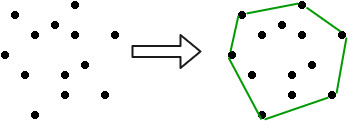
\includegraphics [width=\textwidth]{bab1/img/ilustrasi-convex-hull}
	\caption {Ilustrasi \CH}
	\label {fig:ilustrasi-convex-hull}
\end{figure}


\section {Rumusan Masalah}

Rumusan masalah yang diangkat dalam Tugas Akhir ini adalah sebagai berikut :

\begin {enumerate}
    \item Bagaimana mencari \RCH dari kumpulan titik di dalam sebuah poligon?
    \item Bagaimana algoritma melkman yang dimodifikasi menyelesaikan masalah \RCH dari kumpulan titik?
\end {enumerate}

\section {Batasan Masalah}
\label{sec:batasan_masalah}
Permalsahan yang dibahas pada Tugas Akhit ini memiliki beberapa batasan, yaitu sebagai berikut :
\begin{enumerate}
    \item perbandingan antara algoritma \textit{Multipoint Evaluation} dan \textit{Shifting Evaluation Values} sebagai penyelesaian permasalahan komputasi faktorial pada {Factorial Modulo Prime}.
    \item Implementasi algoritma Melkman yang di modifikasi sebagai penyelesaian permasalahan \RCH pada soal ISUN1.
    \item Algoritma \RCH terbatas pada analisis intuitif yang logis.
\end{enumerate}
Berikut merupakan batasan pada situs \textit{Sphere Online Judge} : 
\begin {enumerate}
\item Implementasi dilakukan menggunakan bahasa pemrograman C++.
    \item Implementasi dilakukan menggunakan bahasa pemrograman C++.
    \item Banyaknya sisi pada poligon pembatas ($n$) diantara 3 sampai 500.
    \item banyaknya pohon yang berada dalam taman ($m$) diantara 0 sampai 500.
    \item Batas maksimum untuk tiap vertex memenuhi($ x $, $ y $) dimana nilai |$x$|, |$y$| $\leq 10000$. 
    \item Banyak soal tidak diketahui karena program berhenti sampai EOF.
    \item Batas waktu yang diberikan adalah $ 0.142 $ detik.
    \item Batas memori yang diberikan adalah $ 1.536 $ MB.
    \item Batas kode sumber yang diberikan adalah $ 50.000 $ B. 
\end {enumerate}

\section {Tujuan}
Tujuan Tugas Akhir ini adalah sebagai berikut :
\begin{enumerate}
    \item Mengevaluasi kinerja algoritma \textit{Multipoint Evaluation} yang diimplementasikan untuk menyelesaikan permasalahan komputasi faktorial pada \textit{Factorial Modulo Prime}.
    \item Mengevaluasi kinerja algoritma \textit{Shifting Evaluation Values} yang diimplementasikan untuk menyelesaikan permasalahan komputasi faktorial pada \textit{Factorial Modulo Prime}.
    \item Melakukan perbandingan algoritma \textit{Multipoint Evaluation} dan \textit{Shifting Evaluation Values} sebagai penyelesaian permasalahan komputasi faktorial pada \textit{Factorial Modulo Prime}.
\end{enumerate}

\section {Manfaat}
Tugas Akhir ini mampu memberikan pemahaman algoritma yang tepat diantara Multipoint Evaluation dan Shifting Evaluation Values dalam menyelesaikan permasalahan komputasi faktorial dalam modulo prima dengan efisien. Dengan komputasi faktorial yang efisien, maka pencarian bilangan prima yang besar untuk RSA akan menjadi efisien juga.

\section {Metodologi}
Metodologi pengerjaan yang digunakan pada Tugas Akhir ini memiliki beberapa tahapan. Tahapan-tahapan tersebut yaitu :

\begin{enumerate}
    \item Penyusunan proposal\\
    Pada tahapan ini penulis memberikan penjelasan mengenai apa yang penulis akan lakukan dan mengapa Tugas Akhir ini dilakukan. Penjelasan tersebut dituliskan dalam bentuk proposal Tugas Akhir.
    \item Studi literatur\\
    Pada tahapan ini penulis mengumpulkan referensi yang diperlukan guna mendukung pengerjaan Tugas Akhir. Referensi yang digunakan dapat berupa hasil penelitian yang sudah pernah dilakukan, buku, artikel internet, atau sumber lain yang bisa dipertanggungjawabkan.
    \item Implementasi algoritma\\
    Pada tahapan ini penulis mulai mengembangkan algoritma yang digunakan untuk menyelesaikan permasalahan komputasi faktorial.
    \item Pengujian dan evaluasi\\
    Pada tahapan ini penulis menguji performa algoritma yang digunakan. Hasil pengujian kemudian dievaluasi untuk kemudian dipertimbangkan apakah algoritma masih bisa ditingkatkan lagi atau tidak.
    \item Penyusunan buku\\
    Pada tahapan ini penulis menyusun hasil pengerjaan Tugas Akhir mengikuti format penulisan Tugas Akhir.
\end{enumerate}

\section {Sistematika Penulisan}
Sistematika laporan Tugas Akhir yang akan digunakan adalah sebagai berikut :
\begin{enumerate}
    \item BABI : PENDAHULUAN\\
    Bab ini berisi latar belakang, rumusan masalah, batasan masalah, tujuan, manfaat, metodologi dan sistematika penulisan Tugas Akhir.
    \item BAB II : DASAR TEORI\\
    Bab ini berisi dasar teori mengenai permasalahan dan algoritma penyelesaian yang digunakan dalam Tugas Akhir
    \item BAB III : DESAIN\\
    Bab ini berisi desain algoritma dan struktur data yang digunakan dalam penyelesaian permasalahan.
    \item BAB IV : IMPLEMENTASI\\
    Bab ini berisi implementasi berdasarkan desain algortima yang telah dilakukan pada tahap desain.
    \item BAB V : UJI COBA DAN EVALUASI\\
    Bab ini berisi uji coba dan evaluasi dari hasil implementasi yang telah dilakukan pada tahap implementasi.
    \item BAB VI : PENUTUP\\
    Bab ini berisi kesimpulan dan saran yang didapat dari hasil uji coba yang telah dilakukan.
\end{enumerate}